\documentclass[a4paper]{report} % doc type is report not exam 
\usepackage{numprint}
\usepackage{hyperref}
\usepackage{graphicx}
\usepackage{amsmath}
\usepackage{diagbox}
\usepackage{dirtytalk}

\graphicspath{{../images/}}
\title{Time Complexity of Cryptographic Algorithms}
\author{  Asad Raza\\
  \texttt{ar06246@st.habib.edu.pk}
  \and
  Batool Ahmed\\
  \texttt{ba06180@st.habib.edu.pk}
  \and 
  Haania Siddiqui\\
  \texttt{hs06188@st.habib.edu.pk}
  \and
  Shamsa Hafeez\\
  \texttt{sd06162@st.habib.edu.pk}
  \and 
  Team: random-path \\}
\date{\today}

\begin{document}
\maketitle

\chapter{Introduction} 

With the rapid expansion in technology, data is shared more frequently than ever. However, it is important to secure this data while sharing information. Encryption is \say{the process of converting human-readable plain text to incomprehensible text, also known as cipher text}
~\cite{cloudflare}. It is the method that scrambles the data and converts plain text to cipher text ~\cite{unknown} Through this way, encryption algorithms ensure that confidentiality of data is maintained and only authorized individuals can read it. ~\cite{unknown}\\

Many encryption algorithms have been developed over the course of several years. Note that an efficient encryption algorithm must not only be difficult to break, but it must also be fast to encrypt. If data encryption algorithm provides high level of security but is very slow at the same time then it might not be of much use in real life applications such as e-commerce, banking, and online transaction processing applications." ~\cite{1598556}\\

This paper discusses the time complexity of the following encryption algorithms: \\ 
\begin{itemize}
    \item Data Encryption Standard (DES) Algorithm 
    \item Blowfish Algorithm 
    \item AES (Advanced Encryion Standard) Algorithm
    \item Hybrid of RSA (Rivest, Shamir, Adleman) Algorithm and AES (Advanced Encryion Standard) Algorithm. 
\end{itemize}

\section{Set Up:}
\begin{itemize}
    \item Python version: 3.9.12
    \item Processor: Intel(R) Core(TM) i5-8250U CPU @ 1.60GHz   1.80 GHz
    \item 64-bit operating system, x64-based processor
    \item RAM: 8.00 GB (7.90 GB usable)
    \item Mode of operation: Electronic Code Block Mode (Details provided in section 1.2.1)
\end{itemize}

\section{Important Terminologies:}
\subsection{Electronic Code Block (ECB) Mode of Operation:} The mode of encryption in which the \say{input plaintext is broken into a number of blocks} ~\cite{CONRAD2016103}. Each block is encrypted separately using the provided key ~\cite{CONRAD2016103}. 
\begin{figure}[h]
\centering
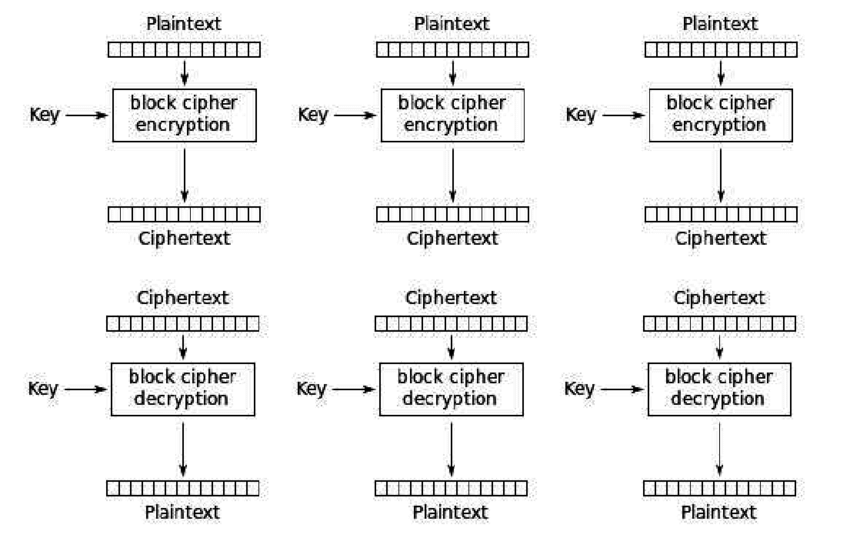
\includegraphics[width=0.7\textwidth]{images/Block-cipher-ECB-mode-operation.png}
\caption{Two Block cipher ECB mode operation ~\cite{Jang}}
\end{figure}

\subsection{Plaintext:} Plaintext refers to \say{anything which humans can understand and/or relate to. This may be as simple as English sentences, a script, or Java code. If you can make sense of what is written, then it is in plaintext} ~\cite{encryptionconsulting}.

\subsection{Ciphertext:} Ciphertext refers to \say{a series of randomized letters and numbers which humans cannot make any sense of. An encryption algorithm takes in a plaintext message, runs the algorithm on the plaintext, and produces a ciphertext} ~\cite{encryptionconsulting}. Ciphertext is also called \textbf{Encrypted Text}.

\subsection{Block Cipher:} An encryption algorithm that \say{works on a fixed-length segment of plaintext data, typically a 64- or 128-bit block as input, and outputs a fixed length ciphertext} ~\cite{CONRAD2016103}. 

\subsection{Types of Encryption:} 
\subsubsection{Symmetric Encryption:} 
\say{In public-key encryption schemes, the encryption key is published for anyone to use and for encrypting messages. Only the receiving party has access to the decryption key that enables messages to be read. Public-key encryption was first described in a secret document in 1973. Before that, all encryption schemes were symmetric-key (also called private-key)} ~\cite{proofpoint}.

\subsubsection{Asymmetric Encryption:} 
\say{In symmetric-key schemes, the encryption and decryption keys are the same. Communicating parties must have the same key in order to achieve secure communication} ~\cite{proofpoint}.

\chapter{Algorithms Analyzed}

\section{Data Encryption Standard (DES) Algorithm:}
\subsection{Introduction:}
In 1970s, the IBM team developed DES (Data Encryption Standard) algorithm and was adopted by the National Institute of Standards and Technology (NIST) ~\cite{simplilearn}.  It is a symmetric-key block cipher. This algorithm takes an input of 64-bit plaintext and 64-bit key and converts it to a 48-bit ciphertext ~\cite{simplilearn}. 



\subsection{Algorithm~\cite{book}~\cite{book1}~\cite{youtube}~\cite{youtube2}~\cite{youtube3}~\cite{youtube4}:}
\begin{center}
    \underline{\textbf{The Key Transformation}}
\end{center}
\begin{enumerate}
    \item The input key is initially of 64 bits 
    \item \textbf{Permuted Choice (PC) 1:} Every $8^{th}$ bit of each byte in the initial key is discarded and the remaining bits are permuted as follows: \\ 
    \begin{figure}[h]
    \centering
    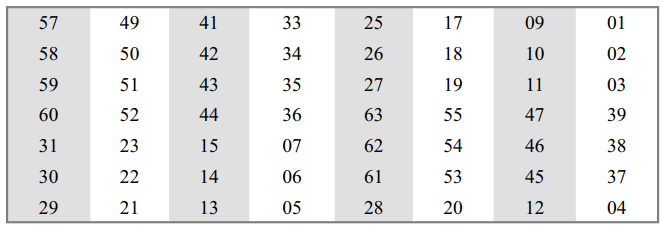
\includegraphics[width=0.7\textwidth]{images/PC1_DES.PNG}
    \caption{PC 1 for Key Transformation }
    \end{figure}\\
    (Note: Now, the remaining steps will change the 56 bits to 48 bits. This is called Key Transformation or Compression Permutation) 
    \item Divide the 56 bits to 2 parts (each of 28 bits). Call them $C_0$ and $D_0$.
    \item Perform a \textbf{Left Circular Shift} to $C_0$ and $D_0$. If the round number is 1, 2, 9 or 16, then left circular shift by 1 bit. For any other round number, left circular shift by 2 bits. 
    \begin{figure}[h]
    \centering
    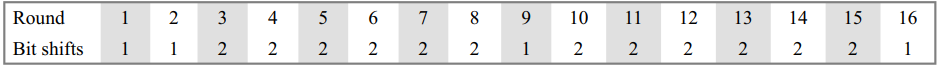
\includegraphics[width=0.7\textwidth]{images/LCS_DES.PNG}
    \caption{Number of bits to left circular shift in each round}
    \end{figure}
    \item Combine $C_0$ and $D_0$. Thus, it makes 56 bits back. 
    \item These 56 bits will now go through \textbf{Permuted Choice 2 (PC 2)}. 48 out of 56 bits are selected and permuted as per the following table. Remaining bits are discarded. \\ 
    \begin{figure}[h]
    \centering
    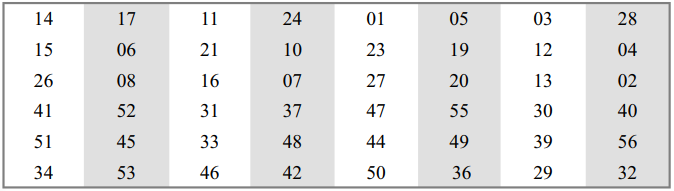
\includegraphics[width=0.7\textwidth]{images/PC2_DES.PNG}
    \caption{PC 2 for Key Transformation }
    \end{figure}
    \item 48 bit key created. Note that 48 bit key is different for each round in DES Algorithm. \\\\
    The key generation is diagrammatically explained below:\\ 
    \begin{figure}[h]
    \centering
    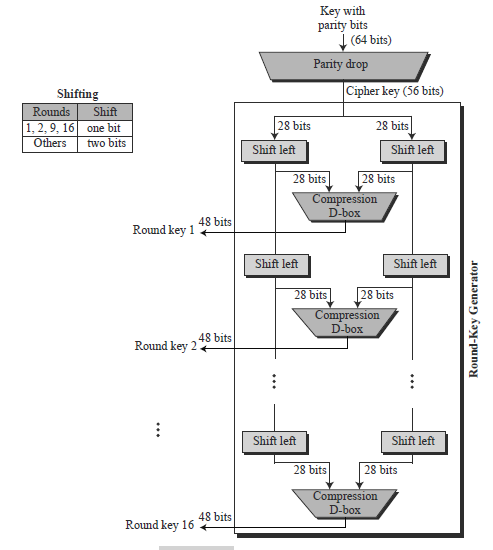
\includegraphics[width=0.6\textwidth]{images/KeyGeneration_DES.PNG}
    \caption{Key Generation for DES}
    \end{figure}
     
\end{enumerate}

\begin{center}
    \underline{\textbf{Main}}
\end{center}
\begin{figure}[h]
\centering
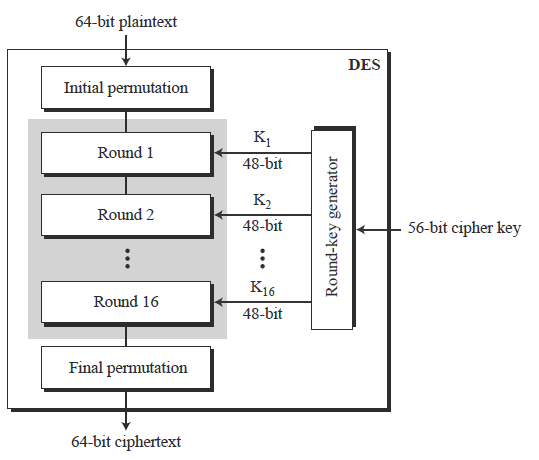
\includegraphics[width=0.7\textwidth]{images/General_DES.PNG}
\caption{Main Algorithm of DES}
\end{figure}

\begin{enumerate}

    \item Plain text of 64 bits is taken as imput 
    \item The \textbf{Initial Permutation} of these 64 bits is done as follows: \\ 
    \begin{figure}[h]
    \centering
    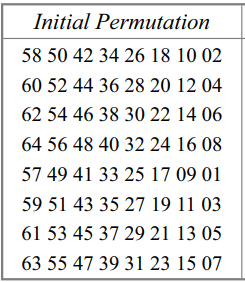
\includegraphics[width=0.35\textwidth]{images/InitialPermutation_DES.PNG}
    \caption{Initial Permutation for DES}
    \end{figure}
    \item The output of Initial Permutation (64 bits) and the 48 bit key of round 1 enters Round 1. Then the output of Round 1 and the 48 bit key of round 2 enters Round 2. This goes on till round 16 as shown in Figure XXX. 
    \item In each round: 
    \begin{enumerate}
        \item Divide the 64 bit input into 2 parts i.e., 32 bits left part (let this be called as $L$) and 32 bits right part (let this be called as $R$)
        \item \textbf{Expansion Permutation on R:} We will do this by dividing it into 8 4-bit sections and each 4-bit section would be expanded to 6-bit section. For each section, input bits 1, 2, 3, and 4 are copied to output bits 2, 3, 4, and 5, respectively. Output bit 1 comes from bit 4 of the previous section; output bit 6 comes from bit 1 of the next section. If sections 1 and 8 can be considered adjacent sections, the same rule applies to bits 1 and 32. \\ 
        \begin{figure}[h]
        \centering
        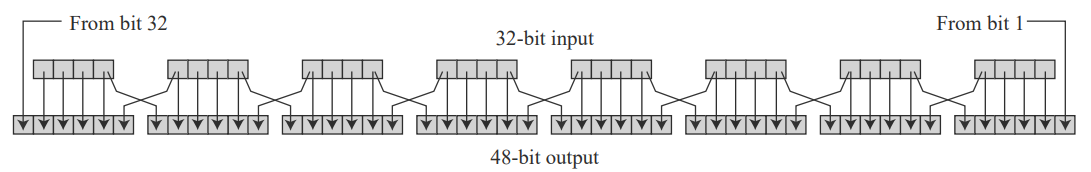
\includegraphics[width=0.8\textwidth]{images/ExpansionPermutation_DES.PNG}
        \caption{Expansion Permutation for DES}
        \end{figure}\\
        Expansion permutation can also be represented as shown in the table below: \\ 
        \begin{figure}[h]
        \centering
        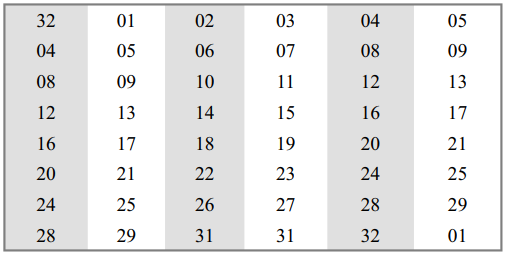
\includegraphics[width=0.6\textwidth]{images/ExpansionTable_DES.PNG}
        \caption{Expansion Table for DES}
        \end{figure}\\
        Thus, now $R$ is of 48 bits
        \item Apply XOR on 48 bits of R and 48 bit Key received for that particular round (Note that each round has a different sub-key). \\
        \item The resulting 48 bits from previous step will now enter the \textbf{Substitution Box (S-box)}
        \begin{itemize}
            \item There will be total 8 S-boxes
            \item 48 bits were recieved from previous step and that can be grouped into 6 group, each of 8 bits
            \item An S-box is basically a table - each table has 4 rows (represented with 2 bits)  and 16 columns (represented with  4-bits). 
            \item Now the 6 bits that are given to S-box as input are split such that the first and the last bit combined represent the row and the bits in between represent the column. 
            \item Go to the given row and the given column of the S-box, take the 4 bit number from there and give it as the output from that particular S-box. 
            \item All 8 S-boxes are given below: 
            \newpage
            \begin{figure}
            \centering
            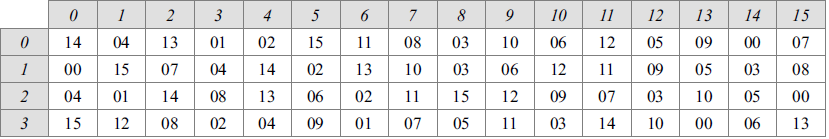
\includegraphics[width=0.9\textwidth]{images/SBox1_DES.PNG}
            \caption{S-Box 1 for DES}
            \end{figure}
        
        \begin{figure}
        \centering
        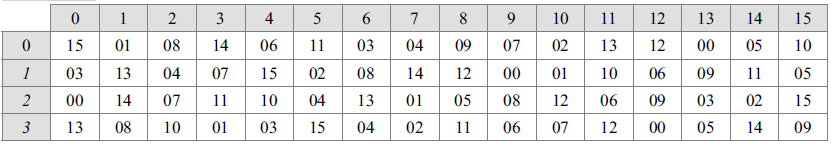
\includegraphics[width=0.9\textwidth]{images/SBox12_DES.PNG}
        \caption{S-Box 2 for DES}
        \end{figure}
        
         \begin{figure}
        \centering
        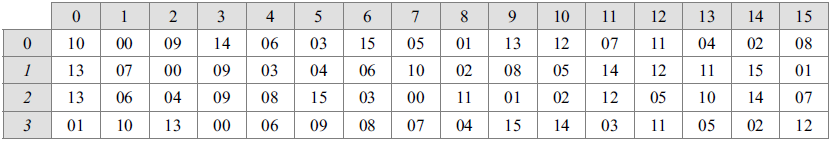
\includegraphics[width=0.9\textwidth]{images/SBox3_DES.PNG}
        \caption{S-Box 3 for DES}
        \end{figure}
        
         \begin{figure}
        \centering
        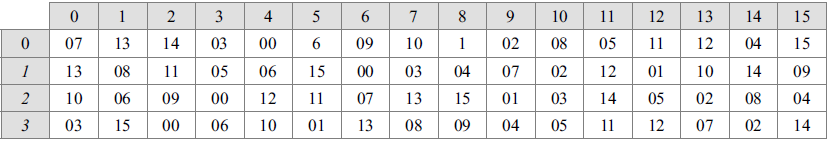
\includegraphics[width=0.9\textwidth]{images/SBox4_DES.PNG}
        \caption{S-Box 4 for DES}
        \end{figure}
         
         \begin{figure}
        \centering
        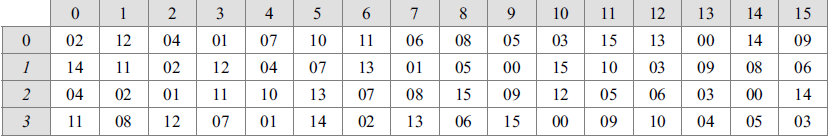
\includegraphics[width=0.9\textwidth]{images/SBox5_DES.PNG}
        \caption{S-Box 5 for DES}
        \end{figure}
        
         \begin{figure}
        \centering
        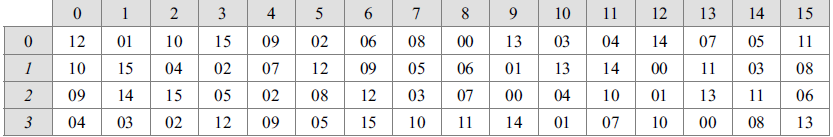
\includegraphics[width=0.9\textwidth]{images/SBox6_DES.PNG}
        \caption{S-Box 6 for DES}
        \end{figure}
        
         \begin{figure}
        \centering
        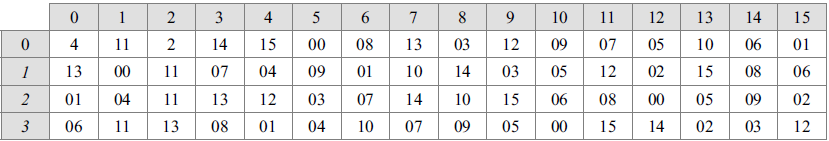
\includegraphics[width=0.9\textwidth]{images/SBox7_DES.PNG}
        \caption{S-Box 7 for DES}
        \end{figure}
         \clearpage 
        \begin{figure}
        \centering
        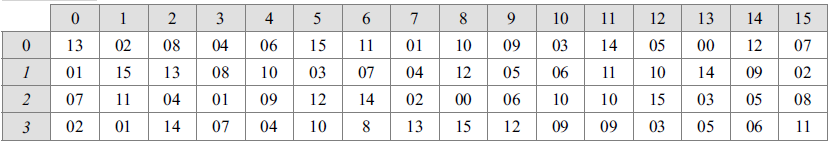
\includegraphics[width=0.9\textwidth]{images/SBox8_7DES.PNG}
        \caption{S-Box 8 for DES}
        \end{figure}
      
        \end{itemize}
        \item Apply Permutation on the resulting 32 bits as given below: \\ 
        \begin{figure}[h]
    \centering
    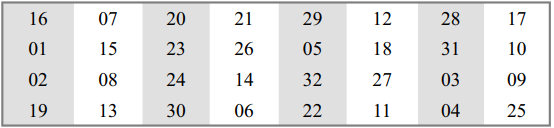
\includegraphics[width=0.35\textwidth]{images/StraightPermutation_DES.PNG}
    \caption{Straight Permutation}
    \end{figure}
    \item Apply XOR on 32-bit $L$ and 32-bits received from previous step. The resulting 32 bits are sent as $R$ to the next round. 
    \item The 32-bits $R$ in step 4(a) is given as $L$ to next round. \\
    \end{enumerate} 
    \item Following is the final permutation : 
    
    \begin{figure}
    \centering
    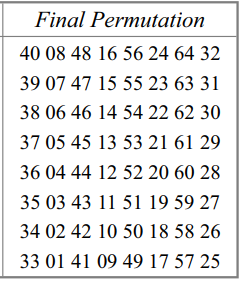
\includegraphics[width=0.3\textwidth]{images/FinalPermutation_DES.PNG}
    \caption{Final permutation for DES}
    \end{figure}
\end{enumerate}

\newpage

\section{Advanced Encryption Standard (AES) Algorithm:}
\subsection{Introduction:} 
AES Encryption algorithm is a symmetric block cipher algorithm which uses block size of 128 bits ~\cite{simplilearn1}. It is also called Rijndael algorithm. It encrypts the blocks of data and forms cipher text using 128, 192, or 256 bits of keys. ~\cite{simplilearn1}

\subsection{Algorithm ~\cite{AES_Lecture}:}

\begin{itemize}
    \item The input is taken as 128 bits in the form a \textbf{State Array} as shown below: 
    \begin{center}
    
    $\begin{bmatrix} \text{byte}_0 & \text{byte}_4 & \text{byte}_8 & \text{byte}_{12} \\ \text{byte}_1 & \text{byte}_5 & \text{byte}_9 & \text{byte}_{13} \\ \text{byte}_2 & \text{byte}_6 & \text{byte}_{10} & \text{byte}_{14} \\ \text{byte}_3 & \text{byte}_7 & \text{byte}_{11} & \text{byte}_{15} 
    \end{bmatrix}$
    \end{center}\\
    
    Notice that the first four bytes of a 128-bit input block occupy the first column in the 4 × 4 array of bytes. The next four bytes occupy the second column, and so on. 
    \item Recall that a \textbf{Word} consists of 4 bytes (32 bits). So, each column of the state array is a word, as is each row. 
    \item Each round of processing works on the input state array and produces an output state array. 
\end{itemize}
\begin{center}
    \textbf{Key and its expansion}
\end{center}
\begin{enumerate}
    \item Assuming a 128-bit key, the key is also arranged in the form of an array of 4 × 4 bytes. As with the input block, the first word from the key fills the first column of the array, and so on.
    \item Now, we will expand the 4 words $w_0, w_1, w_2, w_3$ into 44 words $w_0, w_1, w_2, w_3, w_4, ... , w_{43}$ - so that there are 4 words for the step \textbf{Add Round Key} and 4 word key for each of the 10 rounds. We need to determine the words $w_{i+4}, w_{i+5},  w_{i+6},  w_{i+7}$ from $w_i, w_{i+1}, w_{i+2}, w_{i+3}$ \\
    
    \begin{figure}[ht]
    \centering
    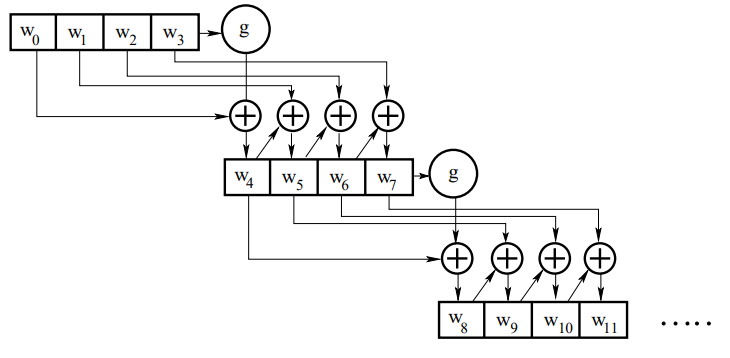
\includegraphics[width=0.6\textwidth]{images/KeyExpansion_AES.PNG}
    \caption{Key Expansion for AES}
    \end{figure}
    \clearpage
    
    \item $w_{i+4} = w_i \otimes g(w_{i+3})$\\ 
    $w_{i+5} = w_{i+4} \otimes w_{i+1}$\\
    $w_{i+6} = w_{i+5} \otimes w_{i+2}$\\
    $w_{i+7} = w_{i+6} \otimes w_{i+3}$\\\\
    Where the function $g()$ consists of following steps:  \begin{itemize}
        \item Perform a one-byte left circular rotation on the argument of g  (which would be a 4-byte word) 
        \item Perform a byte substitution for each byte of the word returned by the previous step by using the same 16 × 16 lookup table as used in the SubBytes step of the encryption rounds.
        \item XOR the bytes obtained from the previous step with \textbf{round constant} 
        \begin{itemize}
            \item Let the Round Constant for $i^{th}$ round be denoted as $Rcon[i]$
            \item $Rcon[i] = (RC[i], 0x00, 0x00, 0x00)$\\
            where , \\ 
            $RC[1] = 0x01$\\
            $RC[j] = 0x02 \times RC[j-1]$
        \end{itemize}
    \end{itemize}
\end{enumerate}
\begin{center}
    \textbf{Main}
\end{center}
\begin{enumerate}
    \item 128 bits are taken as input plain text 
    \item \textbf{Add Round Key} The first four words of the key $w_0, w_1, w_2, w_3$ are bitwise XOR’ed with the input 
    \item Output from previous step enters round 1 along with $w_4, w_5, w_6, w_7$ of the expanded key. Likewise, output of Round 1 enters round 2 with respective 4 words from expanded key and so on. 
    \item After Round 10, Cipher text is finally generated. 
\end{enumerate}
\begin{center}
    \textbf{Rounds in AES}
\end{center}

\begin{figure}[ht]
\centering
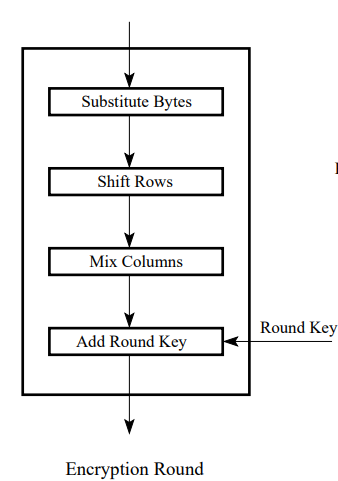
\includegraphics[width=0.3\textwidth]{images/Round_AES.PNG}
\caption{Each round of AES except last round}
\end{figure}

\begin{enumerate}
    \item \textbf{Sub Bytes:} Use the 16 x 16 look-up table to find a replacement byte for a given byte in the input state array. 
    \item \textbf{Shift Rows:}
    \begin{enumerate}
        \item Do not shift the first row of the state array at all
        \item Circularly shift the second row by one byte to the left
        \item Circularly shift the third row by two bytes to the left
        \item Circularly shifting the last row by three bytes to the left.
 
    \end{enumerate}
    \begin{figure}[ht]
    \centering
    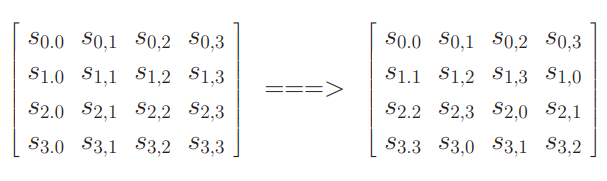
\includegraphics[width=0.7\textwidth]{images/ShiftRows_AES.PNG}
    \caption{Shift Rows for AES}
    \end{figure}
    
    \item \textbf{Mix Columns:} 
    This operation on the state array can be represented in the form of Matrix multiplication as following: 
    
    \begin{figure}[ht]
    \centering
    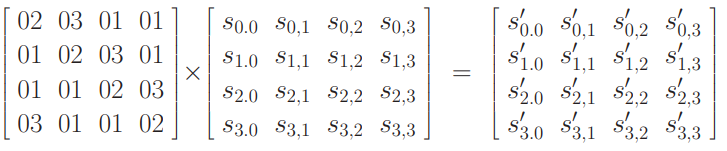
\includegraphics[width=0.7\textwidth]{images/MixColumns_AES.PNG}
    \caption{Mix Columns for AES}
    \end{figure}
    \item \textbf{Add Round Key} Bitwise XOR each byte in state array with the key for that particular round i.e., round key. 
\end{enumerate}
\emph{\textbf{Note: In the last round of AES algorithm, DO NOT perform the Mix Column operation}}
\section{RSA}
\subsection{Introduction:}\\
RSA was invented by Rivest, Shamir and Adleman in year 1978. Hence, the name RSA algorithm. It is an asymmetric cryptography algorithm.The RSA concept is predicated on the fact that factoring a large number is difficult. The public key is made up of two numbers, one of which is the result of multiplying two huge prime numbers. The same two prime numbers are also used to create the private key. As a result, if the huge number can be factored, the private key is compromised. Consequently, RSA's encryption strength is entirely dependent on key size, and as key size is doubled or tripled, encryption strength increases exponentially. RSA keys are normally 1024 or 2048 bits long.\\
\subsection{Algorithm:}\\
There are two sets of keys in this algorithm: private key and public key.The private key is formed using two components, $d$ and $n$ i.e. $(d,n)$, whereas the public key is formed using $e$ and $n$ i.e $(e,n)$.\\
The Algorithm includes the following steps:\\\\
\textbf{Key Generation:}\\
\begin{enumerate}
    \item \textbf{Step 1: Generate RSA Modulus }\\
    \begin{enumerate}
        \item Choose two prime number $p$ and $q$.
        \item Compute $n$ using the formula.\\
        \begin{center}
            $n=p.q$
        \end{center}
        This is the first part of public key and private key. \\
        The reason why the $n$ wasn't chosen directly is because $n$ is large and computation will be complex. This will be discussed in Step 2(a).
    \end{enumerate}
    \item \textbf{Step 2: Derived Number (e)}\\
    \begin{enumerate}
        \item Compute $\phi(n)$ using formula, \\
        \begin{center}
        
        $\phi(n)=\phi(p\times q)=\phi(p)\times \phi(q)=(p-1)\times (q-1)$
        \end{center}
        $\phi(n)$ is used to find $e$ and compute $d$. It is a Euler's quotient function. The formula for $\phi(n)$ when $n$ is a prime number is, \\
        \begin{center}
            $\phi(n)=n-1$
        \end{center}
        This makes the computation less complex because the Euler's function is now applied on two smaller prime numbers rather than a large number. Hence, instead of choosing $n$ directly, two prime numbers were chosen which were factors of $n$. Whenever a quotient function is applied directly on $n$ and that $n$ is not a prime number the process becomes computationally expensive and will take a long time.
        \item Compute $n$ using the formula.\\
        \begin{center}
            $n=p.q$
        \end{center}
        \item Compute $e$ such that, \\
        \begin{center}
        $1\leq e< \phi(n)$ and it is coprime\textsuperscript{1} to $\phi(n)$
        \end{center}
    This is the second part of public key,
    \end{enumerate}
    \item \textbf{Step 3: Public key}\\
     Hence the RSA public key is formed by the computed pair of numbers $n$ and $e$, and it is made public.
    \item \textbf{Step 4: Private Key}\\
    Determine $d$ using multiplicative inverse. Since $e$ and $\phi(n)$ are coprimes, $d$ and $e$ are multiplicative inverse of each other in formula
    \begin{center}
        Since $ed=1 \ mod \ \phi(n) $\\
        $d=e^-1 \ mod \ \phi(n)$
    \end{center}
    Hence, $d$ is also computed. The private key is, \\
    \begin{equation*}
        \text{Private Key}= (d,n)
    \end{equation*}
\end{enumerate}
\footnotetext[1]{Greatest common divisor of $e$ and $\phi(n)$ must be equal to 1}
\textbf{Encryption:}
Consider the case of a sender who sends a plain text($P$) message to a recipient whose public key is $(n,e)$. Use the following syntax to encrypt the plain text message in the current scenario:  
\begin{equation*}
    C = Pe \ mod \ n
\end{equation*}
\section{BlowFish}
\textbf{Introduction:}\\
Blowfish is a symmetric cryptographic algorithm was which created by Bruce Schneier in 1993 as an alternative to the DES Encryption Technique. It is a fast, and free alternative to the existing algorithms, and it uses a variable length key which makes it more secure than the other encryption algorithms. \\\\
\textbf{Algorithm:}\\
There are two parts of this algorithm:\\
\begin{enumerate}
    \item Key Generation
    \item Encryption of the Data
\end{enumerate}
The following are the components of this algorithm: \\
\begin{enumerate}
    \item Input(block size): 64 bits
    \item Key Size: Varies from 32 bits to 448 bits
    \item P-array: Array consisting of 18 subkeys
    \item S-box: 4 Substitution boxes each consisting of 256 entries of size 32 bit each.
    \item Key Array: 14 Keys are stored in an array each of size 32 bit.
    \item Rounds: 16
\end{enumerate}
\textbf{\underline{Key Generation:}}\\
\begin{enumerate}
    \item Break the original input key into a set($k$) of subkeys such that length of this set is 14.
    \begin{center}
        k[0], P[1], P[2]........k[13]

    \end{center}
    \item Initialize a P-array of size 18 (where each subkey is of 32 bit) since 18 subkeys are needed for encryption.
    \begin{center}
        P[0], P[1], P[2]........P[17]
    \end{center}
    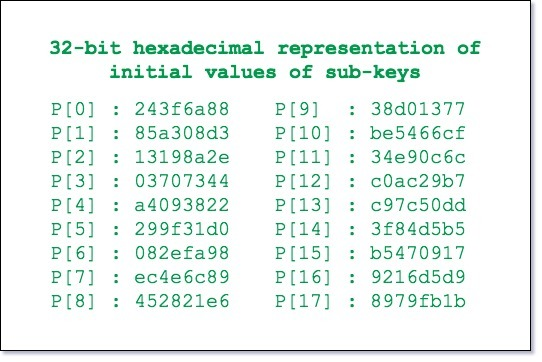
\includegraphics[scale=0.5]{images/Parray.jpg}
    \item Initialize 4 S-boxes. \\
    \begin{center}
        S[0]...S[4]
    \end{center}
    As mentioned earlier, each sub box will have 256 entries.$i^{th}$ box will have\\
    \begin{center}
        S[i][0]......S[i][255] entries
    \end{center}
    \item Initialize each element of P-array and S-box with hexadecimal values
    \item XOR operation is performed between corresponding values of Key and P-arrray.\\
    \begin{equation*}
        P[0]=P[0] \oplus k[0]\\
        .\\
        .\\
        .\\
        P[14]=P[14] \oplus k[14]\\
        P[15]=P[15] \pplus k[0]\\
        .\\
        .\\
        P[17]=P[17] \oplus k[4]\\
    \end{equation*}
    \item Take 64 bit Plain Text where initially all bits are 0. \\
    \begin{center}
        Plain text$[64]=(0,0,0....0)$
    \end{center}
\end{enumerate}
\textbf{\underline{Data Encryption:}}\\
This consists of two parts: Rounds and Post Processing. \\
\underline{Rounds:}\\
There are 16 rounds altogether. Each round takes the plain text from previous round and its corresponding subkey from P-array. Initially the 64 bit plain text is divided into two equal parts and then passed through to rounds. At first, the XOR operation is performed in between left half of the plain text and corresponding subkey from P-array. The result is passed to a function ($F$). Another XOR operation is performed in between output of function and the right half of the plain text. The outputs of both the XOR operations performed in a particular round are passed to the next round as shown in the figure below. \\
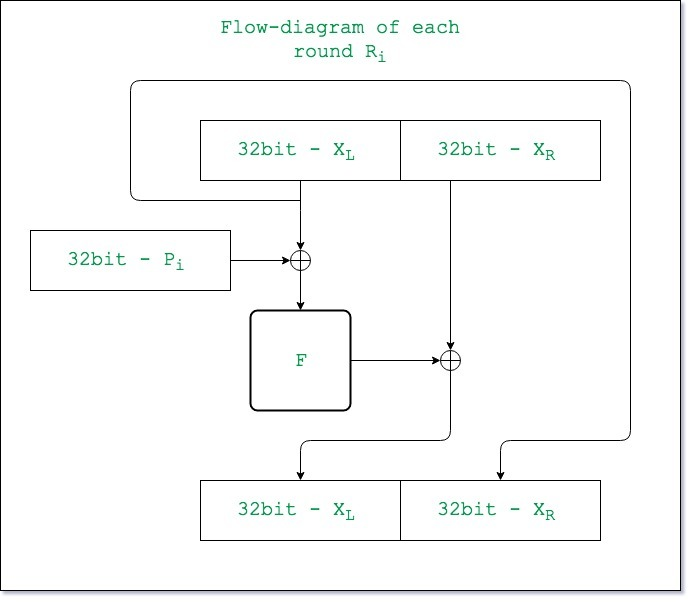
\includegraphics[scale=0.5]{images/round.jpg}\\
The F function divides the 32 bit output from XOR operation into 4 parts and performs the functionality shown in the figure. \\
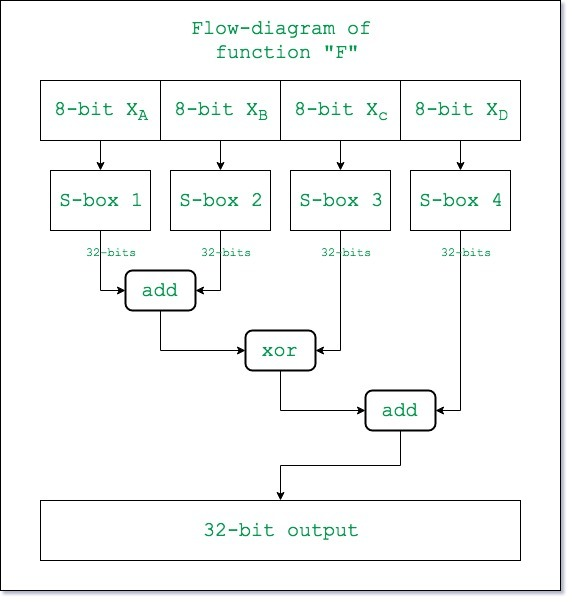
\includegraphics[scale=0.5]{Flow.jpg}\textsuperscript{2}\\
\underline{Post Processing:}\\
After all the rounds have been executed, the outputs from last round are merged and converted into a 64-bit Cipher text.Each new key requires pre-processing that is the equivalent of encrypting around 4 kilobytes of text, which is extremely sluggish when compared to other block ciphers.\\
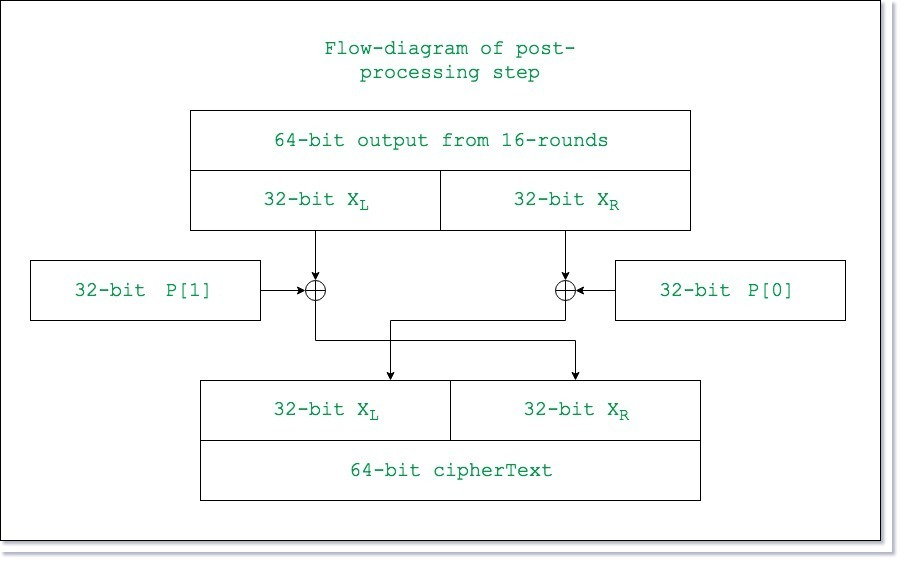
\includegraphics[scale=0.5]{ppr.jpg}\\




\section{Hybrid of AES and RSA:} 
(Ref: \url{https://stackoverflow.com/questions/6309958/encrypting-a-file-with-rsa-in-python})
\begin{enumerate}
    \item Encrypt the data using AES 
    \item Encrypt the Key using in previous step using RSA 
\end{enumerate}
\footnotetext[2]{"add" is addition modulo 2^32}
\chapter{Theoretical Time Complexity:}
\subsection{Big O-Notation:}
\textbf{Analysis:}
\begin{enumerate}
    \item $O(1)$: All of these algorithms are block ciphers and function on a fixed block size and take roughly the same amount of time regardless of input, making them .
    \item $O(m)$ When you use them to encrypt larger messages, the complexity is usually O(m), where $m$ is the message size, because you have blocks of data to encrypt.
    \item Although Blowfish is noted for its slow key scheduling (which can take as long as encrypting 4 KB of data), it is still $O(1)$.
\end{enumerate}
Hence, since their Big-O time complexities are similar, Big-O is not an interesting metric to evaluate these algorithms.However, their speed and strength can vary based on  different input and key sizes. Chapter 4 will cover evaluation of other metrics and their effect on the performance of these algorithms.
\chapter{Empirical Results:} 
Following Diagram represents the analysis generated. Please not that each for the input of 0.5 MB,1 MB,2 MB,5 MB, 10 MB and 20 MB files, we took an average of 3 iterations: \\ 
\begin{center}
 \npdecimalsign{.}
\nprounddigits{3}
\begin{tabular}{ |c|n{5}{2}|n{5}{2}|n{5}{2}|n{5}{2}|n{5}{2}|n{5}{2}|} 
 \hline

 \backslashbox{Algorithm}{File Size(MB)} & \text{0.5} & 1 & 2 & 5 & 10 & 20  \\ 
 \hline 
 DES & 56.07155307133993 & 155.30495127042136 & 300.83055329322815 & 683.6926143964132 & 1394.9095814228058 & 1491.864587386449  \\ 
 \hline 
 Hbrid of RSA and AES & 0.39353783925374347 & 0.40140334765116376  & 0.5879687468210856 & 0.33449244499206543 & 0.7293424606323242 & 0.4185202121734619  \\ 
 \hline 
 Blowfish & 0.010855913162231445 &  0.02772410710652669 & 0.04418683052062988 & 0.1013654073079427 & 0.2271113395690918 & 0.23474876085917154\\ 
 \hline 
 AES & 0.006975332895914714 & 0.004294157028198242 & 0.006531715393066406 & 0.01970958709716797 & 0.04281433423360189 & 0.0458830197652181\\
 \hline
\end{tabular}
\end{center}

%%%%%%%%%%%%%%%%%
\begin{figure}[ht]
\centering
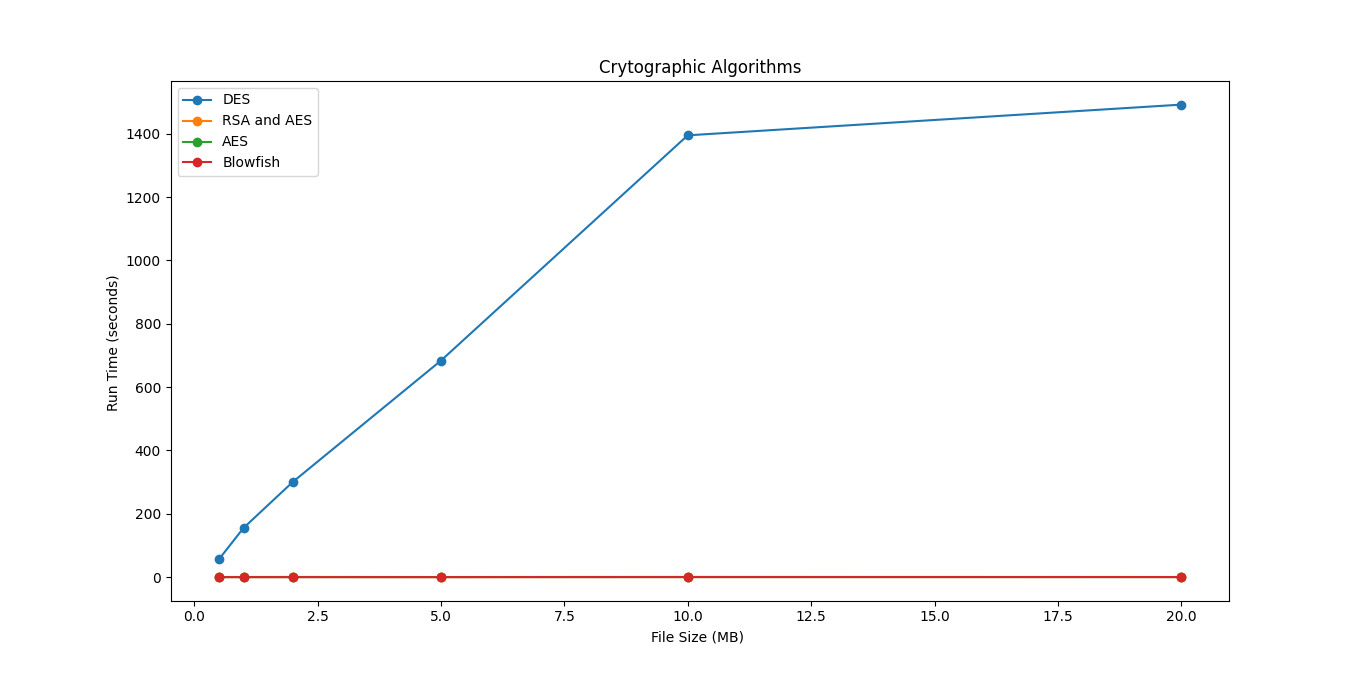
\includegraphics[width=1\textwidth]{images/FINAL.png}
\caption{Run Time for each of the Cryptographic algorithms on 0.5 MB,1 MB,2 MB,5 MB, 10 MB and 20 MB files}
\end{figure}

\begin{figure}
\centering
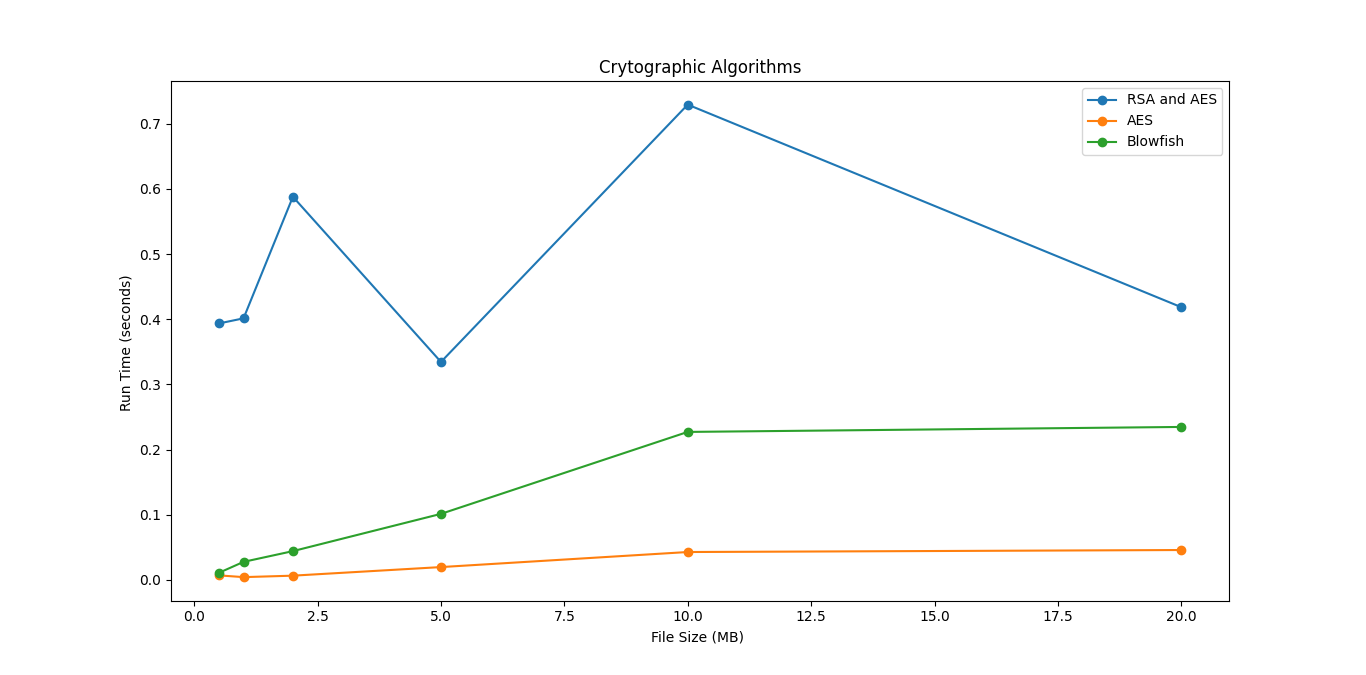
\includegraphics[width=1\textwidth]{images/Final1.png}
\caption{Run Time for each of the hybrid of AES and RSA, Blowfish and AES algorithms on 0.5 MB,1 MB,2 MB,5 MB, 10 MB and 20 MB files}
\end{figure}
    


Since hybrid of AES and RSA, Blowfish and RSA were so close. We ran these algorithms again. This time, we tested for files of 5MB, 10MB, 15MB, 20MB, 25MB, 30 MB, 35MB, 40MB, 45MB and 50MB. The run time plotted on graph was an average of 100 iterations. 


\begin{figure}
\centering
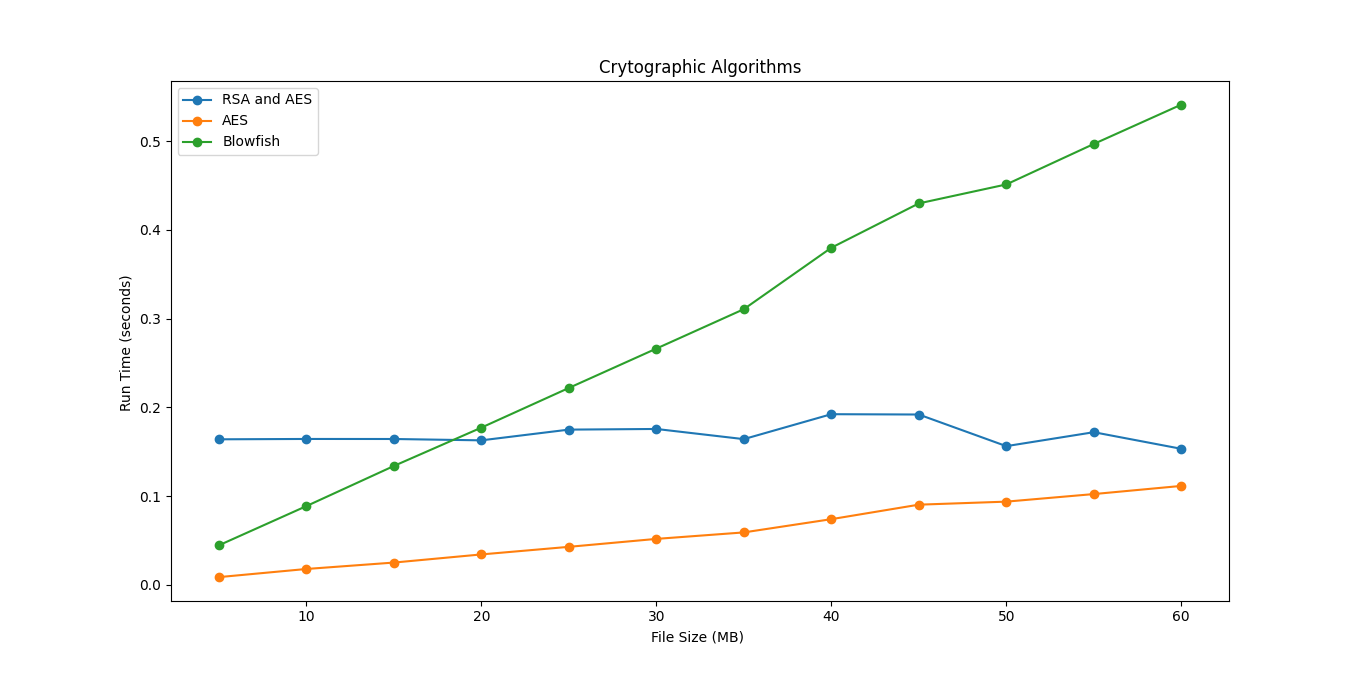
\includegraphics[width=1\textwidth]{images/three.png}
\caption{Run time of hybrid of AES and RSA, Blowfish and RSA on 5MB, 10MB, 15MB, 20MB, 25MB, 30 MB, 35MB, 40MB, 45MB and 50MB files}
\end{figure}

\clearpage
\section{Analysis:}
\textbf{Theoretical Analysis:}\\
The preference of cryptographic algorithms is based on their strength which is based on a number of parameters that impact how much effort is required to encrypt the text and convert it into a cipher text. We looked at six different factors that  differentiate between the four Encryption  ciphers as part of our theoretical comparison analysis. The parameters are as follows:
\begin{enumerate}
    \item Cipher key length: The length of the cipher's key in each round.
    \item Rounds: How many times the primary function was performed.
    \item Block Size (in bits): The size of the text input block.
    \item Security Level: How much impenetrable it is?
    \item Attacks Found: Number of successful attacks
    \item Hardware acceleration
\end{enumerate}
\textbf{Hardware acceleration and RAM:}
    AES includes hardware acceleration\textsuperscript{3} which means that it is fast while still being secure against cache-timing attacks.Blowfish, on the other hand, does not have hardware acceleration.\\
    AES is a popular encryption solution because of its low RAM requirements and great speed. It also works well on a variety of hardware, ranging from little chip cards to high-end systems.\\ \\
\textbf{Key Size:}
In terms of security level and number of attacks, Blowfish is better because it uses variable length key size which makes it most secure. The worst in terms of key length is DES, it is insufficiently secure because it is easily crackable due to its small key length and brute force attacks.\\ \\
\textbf{Block Size}
Blowfish uses the size of 64 bits whereas AES uses larger bit size-128 bits, that makes it better for encryption than Blowfish. A severe security issue is it's block size; Blowfish is more vulnerable to birthday attacks\textsuperscript{4} as a result of its small block size.\\ \\ \textbf{Rounds:}
One reason why RSA is less secure than other algorithms because ot it's number of rounds.Rounds are defined as a complete unit of encryption or decryption operations applied to plaintext or cypher text, respectively. This unit is repeated a certain number of times in order to strengthen the strength of function being performed on text. RSA is the only one of the four that does not use this method, as it involves performing a series of mathematical functions all at once. \\ \\ 
\textbf{Empirical Analysis:}\\
It can be inferred from the empirical analysis that among the  ciphers, AES had the highest speed whereas Blowfish was the second fastest algorithm. Moreover, we observed that the Hybrid Model i.e. combining the RSA and AES affected the performance of AES negatively and the execution time increased as compared to AES algorithm. AES and blowfish both work fast due to their bulk encryption. 
Our results also showed that key size isn't necessarily a reliable indicator of key strength. BlowFish  supports up to 448-bit keys and AES supports up to 256-bit keys and still AES performs better in terms of speed.\\ \\
Although, we were expecting Blowfish to be faster than AES because of it's variable key length and bulk encryption but it can be observed that according to theoretical analysis, this result is also justified. Due to the limitations of our hardware, AES was able to perform better than Blowfish.Moreover, it has a larger block size which makes it better for bulk encryption than Blowfish and other encryption algorithms.

\footnotetext[3]{Hardware acceleration is the use of computer hardware designed to perform specific functions more efficiently when compared to software running on a general-purpose central processing unit}
\footnotetext[4]{Birthday attack is a type of cryptographic attack that belongs to a class of brute force attacks}

\section{Limitations:}
The limitations were primarily those of available hardware, including the processor and RAM, as well time constraint. Moreover, since our computer could not run the RSA encryption algorithm for the file sizes we have considered within a set time constraint, we had to switch to a hybrid RSA-AES algorithm instead. Furthermore, limitations on processing power also acted as a barrier to considering even larger file sizes for the analysis. 
\section{Conclusion:}
As AES is faster, performs bulk encryption and has a greater block sizes, which makes it less susceptible to attacks, this is to conclude that AES is more effective than Blowfish, RSA and AES-RSA under all scenarios and limitations. Moreover, block size of an algorithm is a better evaluation metric. In addition to that, it is critical not to concentrate solely on the key size, but also to examine other properties of algorithms that affects it's speed and strength. In conclusion, AES is the best encryption algorithm.

\section{Future Prospects:}
\begin{enumerate}
    \item The scope of this paper was limited to ECB mode, however, further research can be done on the efficiency of cryptographic algorithms with respect to time in other modes of operations (for example. 
    \item Only 4 techniques were evaluated as a part of this paper. There are many other encryption algorithms that can be analyzed (including DES3, RSA, SHA etc) 
    
\end{enumerate}
\bibliographystyle{acm}
\bibliography{refs.bib}
\end{document}
